\documentclass[aspectratio=169,11pt]{beamer}
\usepackage[T1]{fontenc}
\usepackage{lmodern,booktabs,tikz}
\usetikzlibrary{positioning,arrows.meta}
\definecolor{navy}{HTML}{142D4E}
\definecolor{teal}{HTML}{007F86}
\usetheme{Madrid}
\setbeamercolor{structure}{fg=teal}
\setbeamercolor{frametitle}{bg=navy,fg=white}
\setbeamercolor{title}{bg=navy,fg=white}
\setbeamertemplate{navigation symbols}{}
\setbeamertemplate{footline}{\hspace{1em}\scriptsize Phoenix Rebirth\hfill Farhan Tanvir Utshaw\hfill\insertframenumber\hspace{1em}\vskip5pt}
\setbeameroption{hide notes}
% Change hide notes to show notes to compile the rehearsal version.
\newcommand{\src}[1]{\vfill{\tiny\color{gray}Source: Yoo, Romano, and Kozyrakis (2009), #1.}}
\title{Phoenix Rebirth}
\subtitle{Scalable MapReduce on a Large-Scale Shared-Memory System}
\author{Farhan Tanvir Utshaw}
\institute{Missouri State University\\Class paper presentation}
\date{}
\begin{document}
\begin{frame}
\titlepage
\vspace{-1em}\centering\small Paper by Richard M. Yoo, Anthony Romano, and Christos Kozyrakis\\Stanford University, 2009
\note{[0:00--0:25] This paper asks why a parallel data-processing runtime can stop getting faster even when hundreds of hardware threads are available. Phoenix implements MapReduce inside one shared-memory machine. The authors show that making it scale requires coordinated changes across the runtime and its interactions with the operating system.}
\end{frame}

\begin{frame}{The problem: more threads can mean less performance}
\begin{columns}[T]
\column{.55\textwidth}
\begin{itemize}
\item Original Phoenix targeted smaller shared-memory machines.
\item On the larger NUMA system, no tested application scaled beyond 64 threads.
\item Most slowed down as more threads were added.
\end{itemize}
\column{.41\textwidth}
\begin{block}{Research question}
How can a runtime preserve locality and avoid contention as it crosses chip boundaries?
\end{block}
\end{columns}
\begin{alertblock}{Central claim}
Scalability requires attention to algorithms, data structures, and OS services together.
\end{alertblock}
\src{Sections I--II; Fig. 1}
\note{[0:25--1:10] The original design worked reasonably well at smaller scale. The surprising observation is that adding workers beyond one chip often hurts. This is not simply a shortage of parallel work. Workers can compete over memory, synchronization, and operating-system mechanisms. The paper investigates where those costs originate and fixes them at three layers.}
\end{frame}

\begin{frame}{Phoenix: MapReduce within one address space}
\centering
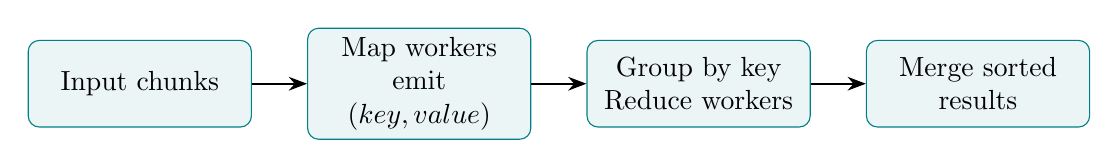
\begin{tikzpicture}[node distance=7mm,box/.style={draw=teal,rounded corners,fill=teal!8,text width=2.6cm,minimum height=1.1cm,align=center},>=Stealth]
\node[box] (a) {Input chunks};
\node[box,right=of a] (b) {Map workers\\emit $(key,value)$};
\node[box,right=of b] (c) {Group by key\\Reduce workers};
\node[box,right=of c] (d) {Merge sorted\\results};
\draw[->,thick] (a)--(b);\draw[->,thick] (b)--(c);\draw[->,thick] (c)--(d);
\end{tikzpicture}
\vspace{.5cm}
\begin{exampleblock}{Word-count example}
\texttt{cat dog cat} $\rightarrow$ $(cat,1),(dog,1),(cat,1)$\\
Group $cat:[1,1],\ dog:[1]$ $\rightarrow$ $(cat,2),(dog,1)$.
\end{exampleblock}
\begin{itemize}
\item Programmer supplies map and reduce functions.
\item Runtime manages worker threads and intermediate data in shared memory.
\item Shared memory avoids network communication, but introduces shared-resource contention.
\end{itemize}
\src{Section II-A; example is illustrative}
\note{[1:10--2:00] Briefly explain map and reduce through word count. Each occurrence emits one pair; reduction combines values for the same key. Unlike cluster MapReduce, these workers are threads in a single process, and intermediate pairs stay in memory. Communication is cheap, but all threads also depend on the same address-space management. That distinction becomes crucial later.}
\end{frame}

\begin{frame}{NUMA: shared memory does not mean equal access cost}
\begin{columns}[T]
\column{.5\textwidth}
\begin{block}{Experimental platform}
\begin{itemize}
\item Sun SPARC Enterprise T5440
\item 4 chips $\times$ 8 cores $\times$ 8 hardware contexts = 256 threads
\item 128 GB memory; Solaris 5.10
\item Threads fill one chip before the next
\end{itemize}
\end{block}
\column{.46\textwidth}
\centering
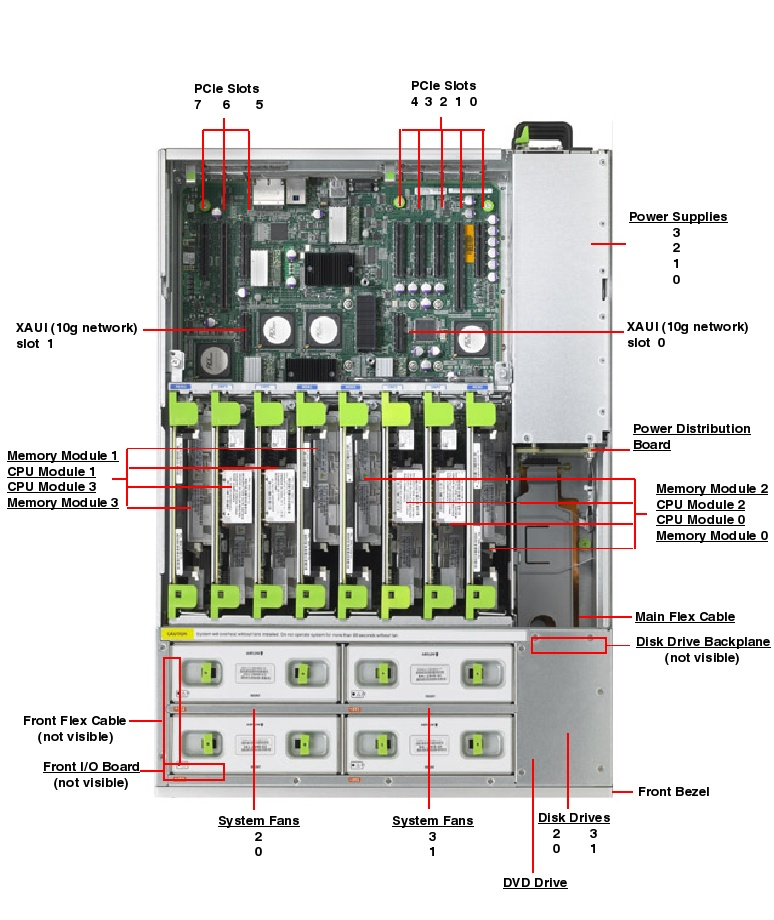
\includegraphics[width=\linewidth,height=4.2cm,keepaspectratio,trim=0bp 150bp 0bp 80bp,clip]{assets/SE_T5440_top_callout.jpg}\\[-.1cm]
{\scriptsize Actual four-socket T5440 platform: CPU and memory modules.}
\end{columns}
\vspace{.3cm}
\textbf{NUMA} = non-uniform memory access. Remote DRAM access costs about 33\% more on this machine.
\src{Section II-B; Table I. Platform photo: Sun SPARC Enterprise T5440 System Handbook.}
\note{[2:00--2:50] Distinguish cores from hardware contexts: this is 32 cores and 256 hardware threads, not 256 cores. Each chip has nearby memory, while other memory is farther away. Local latency is approximately 300 cycles and remote adds 100. At more than 64 workers, execution crosses chips under the experiment's placement policy. Scheduling and allocation must therefore consider where data lives.}
\end{frame}

\begin{frame}{Layer 1: schedule work near its input data}
\begin{enumerate}
\item Maintain one task queue per \textbf{locality group} (chip and local memory).
\item Place map tasks according to the location of their input chunks.
\item Workers consume local tasks first.
\item When local work runs out, steal from a remote queue.
\end{enumerate}
\begin{block}{Why keep stealing?}
Locality reduces remote traffic; stealing prevents idle workers when queues are uneven.
\end{block}
\textbf{Evidence:} string-match local-memory hit rate reached 44\% at 256 threads; the paper reports an average 8\% speedup improvement from this optimization at 256 threads.
\src{Sections III-A and IV-B; Fig. 5}
\note{[2:50--3:40] A locality group is a chip together with its nearby memory. Queue placement connects tasks to data location, rather than treating every worker as interchangeable. Strict locality alone could leave some chips idle, so remote stealing balances the load. The gain is useful but modest: locality-aware scheduling alone does not explain the paper's headline improvement.}
\end{frame}

\begin{frame}{Layer 2: make intermediate data cheaper to grow}
\small
\begin{columns}[T,onlytextwidth]
\column{.55\textwidth}
\centering
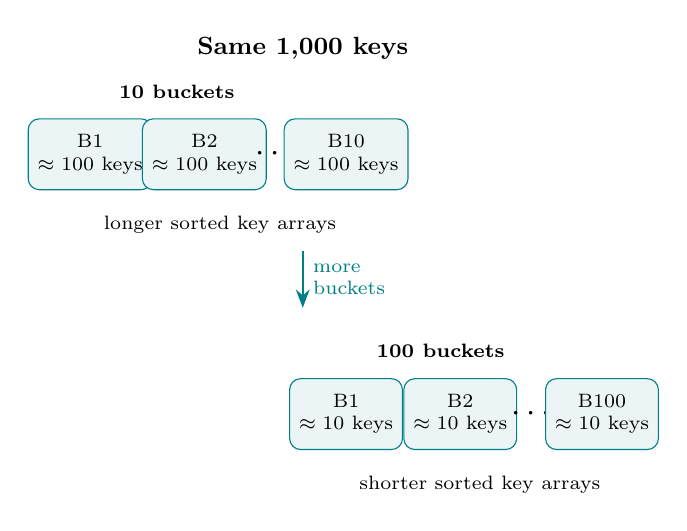
\begin{tikzpicture}[bucket/.style={draw=teal,rounded corners,fill=teal!8,minimum width=1.35cm,minimum height=.9cm,align=center,font=\scriptsize},>=Stealth]
\node[font=\small\bfseries] at (2.7,3.2) {Same 1,000 keys};
\node[font=\scriptsize\bfseries] at (1.1,2.65) {10 buckets};
\node[bucket] (a1) at (0,1.85) {B1\\$\approx100$ keys};
\node[bucket] (a2) at (1.45,1.85) {B2\\$\approx100$ keys};
\node[font=\large] at (2.35,1.85) {$\cdots$};
\node[bucket] (a3) at (3.25,1.85) {B10\\$\approx100$ keys};
\node[font=\scriptsize] at (1.65,.95) {longer sorted key arrays};
\draw[->,thick,teal] (2.7,.62)--node[right,font=\scriptsize,align=left]{more\\buckets}(2.7,-.1);
\node[font=\scriptsize\bfseries] at (4.45,-.65) {100 buckets};
\node[bucket] (b1) at (3.25,-1.45) {B1\\$\approx10$ keys};
\node[bucket] (b2) at (4.7,-1.45) {B2\\$\approx10$ keys};
\node[font=\large] at (5.6,-1.45) {$\cdots$};
\node[bucket] (b3) at (6.5,-1.45) {B100\\$\approx10$ keys};
\node[font=\scriptsize] at (4.95,-2.35) {shorter sorted key arrays};
\end{tikzpicture}
\column{.42\textwidth}
\begin{block}{Why this helps}
\begin{itemize}
\item Sorted keys support binary lookup in $O(\log k)$.
\item A new key can shift later keys: $O(k)$.
\item Lower $k$ means fewer shifts, smaller resizes, and less copying.
\end{itemize}
\end{block}
\begin{alertblock}{Tradeoff}
Keys stay sorted, but more buckets add traversal and merge work. Tune the count to the workload.
\end{alertblock}
\end{columns}
\src{Sections III-B and IV-C1; Figs. 3, 6--7}
\note{[3:40--4:20] The map phase can produce a huge number of intermediate pairs such as $(cat,1)$ and $(dog,1)$. Phoenix must keep those pairs until reduce runs. Each bucket stores its keys in sorted order so the runtime can quickly check whether an incoming key already exists. For example, with $[apple, banana, orange, pear]$, it can locate $orange$ with binary search in $O(\log k)$ rather than scanning an unsorted array in $O(k)$, where $k$ is the number of keys in that bucket. The tradeoff is insertion. A new key must preserve the sorted order, so it can shift later keys, which costs $O(k)$. A full key array can also require a larger allocation and a copy of its contents. Phoenix Rebirth increases the number of hash buckets, making each sorted array smaller and reducing those shifts and resizes. The keys remain sorted. But more buckets create traversal and merge work, so the best count depends on the workload's number of unique keys.}
\end{frame}

\begin{frame}{Layer 2: grow values without copying}
\begin{columns}[T,onlytextwidth]
\column{.43\textwidth}
\centering\textbf{Original: one contiguous array}\\[.25cm]
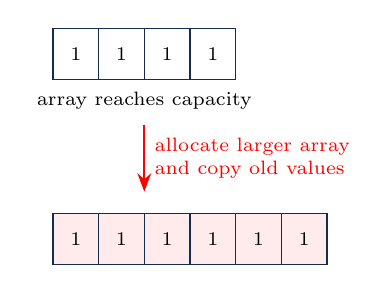
\begin{tikzpicture}[cell/.style={draw=navy,minimum width=.58cm,minimum height=.65cm,align=center,font=\scriptsize},>=Stealth]
\foreach \x/\v in {0/1,.58/1,1.16/1,1.74/1} \node[cell] at (\x,1.2) {\v};
\node[font=\scriptsize] at (.87,.6) {array reaches capacity};
\draw[->,thick,red] (.87,.3)--node[right,font=\scriptsize,align=left]{allocate larger array\\and copy old values}(.87,-.55);
\foreach \x/\v in {0/1,.58/1,1.16/1,1.74/1,2.32/1,2.9/1} \node[cell,fill=red!8] at (\x,-1.15) {\v};
\end{tikzpicture}
\column{.53\textwidth}
\centering\textbf{Phoenix Rebirth: linked chunks}\\[.25cm]
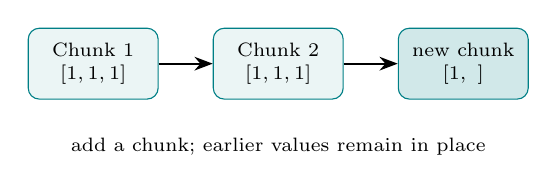
\begin{tikzpicture}[chunk/.style={draw=teal,rounded corners,fill=teal!8,minimum width=1.65cm,minimum height=.9cm,align=center,font=\scriptsize},>=Stealth]
\node[chunk] (c1) at (0,0) {Chunk 1\\$[1,1,1]$};
\node[chunk] (c2) at (2.35,0) {Chunk 2\\$[1,1,1]$};
\node[chunk,fill=teal!18] (c3) at (4.7,0) {new chunk\\$[1,\ ]$};
\draw[->,thick] (c1)--(c2);
\draw[->,thick] (c2)--(c3);
\node[font=\scriptsize,align=center] at (2.35,-1.05) {add a chunk; earlier values remain in place};
\end{tikzpicture}
\end{columns}
\vspace{.25cm}
\begin{block}{Result}
Adding capacity attaches a new chunk rather than copying the full value list. A sequential iterator lets reduce read all chunks as one values stream.
\end{block}
\src{Section III-B; Fig. 3}
\note{[4:20--4:45] The keys identify groups, but the values associated with one key also have to grow. The original contiguous array was simple, yet a full array required a larger allocation and a copy of its old contents. Phoenix Rebirth breaks the values into chunks. Adding capacity means linking a new chunk, not moving all old values. The reduce function still sees one sequential stream through an iterator, so the storage optimization does not complicate its interface.}
\end{frame}

\begin{frame}{Layer 2: remote reduce access}
\begin{block}{Why reduce can access remote memory}
Map tasks on different chips can emit values for the same key. The key's values may therefore reside in more than one locality group.
\end{block}
\begin{alertblock}{The cost}
Reduce must visit all values for that key. Remote reads take longer than local reads, so irregular access can stall the worker.
\end{alertblock}
\begin{block}{Phoenix Rebirth: sequential iteration and prefetching}
\begin{itemize}
\item The chunk iterator reads values in sequence instead of chasing scattered locations.
\item Prefetching requests the next data before reduce needs it.
\item This hides some latency, but values can still require remote access.
\end{itemize}
\end{block}
\src{Section III-B; Figs. 3 and 7}
\note{[4:45--5:10] More buckets and chunks help data growth, but a reduce task can still require values produced on more than one chip. That creates remote-memory reads. Phoenix exposes values through a sequential iterator, then prefetches the next chunk or values before the reducer consumes them. This can hide part of the latency. It does not guarantee that every reduce access becomes local.}
\end{frame}

\begin{frame}{Layer 3: reuse threads to reduce OS overhead}
\begin{itemize}
\item Repeatedly creating and joining workers allocates and destroys thread stacks.
\item Stack cleanup invokes \texttt{munmap()}, which becomes expensive at high thread counts.
\item A \textbf{thread pool} reuses workers across phases and iterations.
\end{itemize}
\begin{block}{Measured effect on k-means at 256 threads}
\centering
\begin{tabular}{lrr}
\toprule & Without pool & With pool\\\midrule
\texttt{munmap()} calls & 14,697 & 102\\
Time in \texttt{munmap()} & 8.219 s & 0.065 s\\\bottomrule
\end{tabular}
\end{block}
\textbf{Interpretation:} reduce how often the costly service is called; the service itself is not made faster.
\src{Sections III-C and IV-D; Table IV}
\note{[5:10--6:05] Iterative k-means repeatedly executes MapReduce, making thread lifecycle costs especially visible. The pool keeps workers alive between phases and iterations. This dramatically reduces stack-unmapping calls. These numbers measure time in munmap, not total application runtime. The per-call cost does not improve, so the runtime is avoiding a bottleneck rather than fixing the operating system.}
\end{frame}

\begin{frame}{Evaluation: compare the same workloads and datasets}
\small
\begin{tabular}{ll}
\toprule Workload & Input\\\midrule
Histogram & 1.4 GB BMP image\\
K-means & 500,000 data points\\
Linear regression & 3.5 GB data\\
Matrix multiplication & $3{,}000\times3{,}000$ matrices\\
Principal components analysis & $3{,}000\times3{,}000$ matrix\\
String matching & 500 MB dictionary\\
Word count & 500 MB random text\\\bottomrule
\end{tabular}
\vspace{.3cm}
\begin{itemize}
\item Larger datasets stress the available hardware contexts.
\item Original and optimized runtimes compared across 1--256 threads.
\item Reverse index excluded because it was I/O bound.
\end{itemize}
\src{Section IV-A; Table II}
\note{[6:05--6:45] The evaluation covers seven workloads, including text processing and numerical computation. Do not read every row aloud. Emphasize that the datasets were enlarged relative to the original Phoenix study, and that both runtime versions use the same datasets in the comparison. The excluded I/O-bound workload is a useful limitation to remember when interpreting generality.}
\end{frame}

\begin{frame}{Results: substantial improvement, but not universal scaling}
\begin{columns}[T,onlytextwidth]
\column{.60\textwidth}
\centering
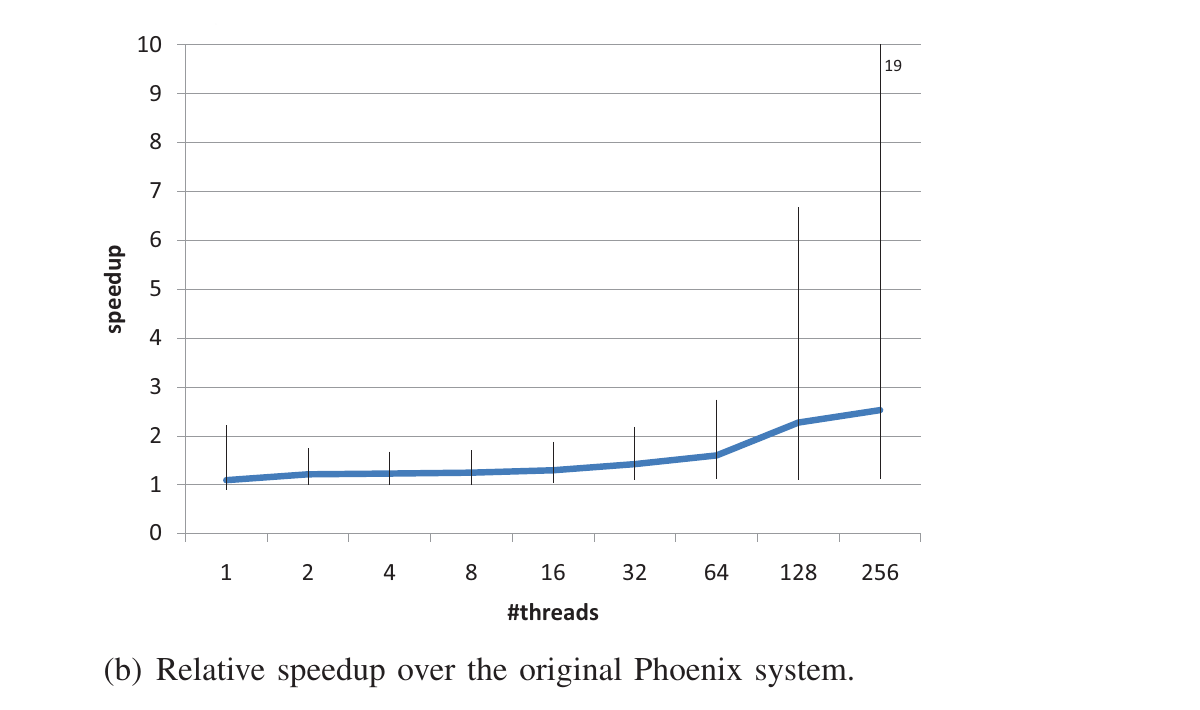
\includegraphics[width=.96\linewidth]{assets/phoenix-fig4b-clean.png}
\column{.36\textwidth}
\begin{block}{At 256 threads}
\centering\Large $\mathbf{2.5\times}$\\[-.05cm]\scriptsize harmonic-mean improvement\\[.2cm]
\Large $\mathbf{19\times}$\\[-.05cm]\scriptsize maximum improvement
\end{block}
\textbf{Scaled through 256 threads:}
\begin{itemize}
\item Matrix multiplication
\item K-means
\item PCA
\item String matching
\end{itemize}
\textbf{Still limited:} histogram, linear regression, and word count.
\end{columns}
\vspace{-.1cm}
\src{Abstract; Section IV-A; Fig. 4(b)}
\note{[6:45--7:45] Be precise about the denominator. The headline compares optimized Phoenix with original Phoenix at the same thread count. It does not mean a 19-times speedup over serial execution for every application. The aggregate is a harmonic mean, rounded to about 2.5 in the headline. Four workloads scale across the entire system, while three still fail to do so. The paper qualitatively finds OS interaction changes most influential, followed by implementation and scheduling changes, but their effects interact.}
\end{frame}

\begin{frame}{Why three workloads still stop scaling}
\begin{columns}[T]
\column{.48\textwidth}
\begin{block}{Memory allocation}
Many intermediate pairs create allocation pressure. Parallel allocators still depend on \texttt{sbrk()} scalability.\\[.2cm]
Word count spent 28\% of execution time in \texttt{sbrk()} at 256 threads.
\end{block}
\column{.48\textwidth}
\begin{block}{Mapped-input page faults}
Threads share one address space; concurrent access to mapped input can expose OS serialization.\\[.2cm]
Histogram and linear regression spent 64\% and 63\% idling for data page faults.
\end{block}
\end{columns}
\begin{alertblock}{Diagnostic experiment}
Pre-allocating memory and reading input before execution allowed a synthetic word-count experiment to scale through 256 threads.
\end{alertblock}
\src{Section V; Figs. 10--14}
\note{[7:45--8:45] After runtime improvements, the OS becomes visible as the remaining limit. Allocation and mapped-file page faults affect threads sharing one address space. A synthetic experiment removes both effects from the measured work and recovers scaling. This supports the bottleneck explanation, but moving work before the timed region is not a free end-to-end optimization. It is diagnostic evidence about what limits the runtime.}
\end{frame}

\begin{frame}{Critical assessment}
\begin{columns}[T]
\column{.48\textwidth}
\begin{block}{Strengths}
\begin{itemize}
\item Connects performance to concrete mechanisms.
\item Combines application results, profiling, and microbenchmarks.
\item Explains why plausible changes can backfire.
\end{itemize}
\end{block}
\column{.48\textwidth}
\begin{block}{Limits}
\begin{itemize}
\item Main evidence is one historical platform and OS.
\item Workload-specific tuning is required.
\item Interacting changes prevent complete attribution of gains.
\end{itemize}
\end{block}
\end{columns}
\vspace{.3cm}
\textbf{My interpretation:} the mechanisms are broadly instructive; the numerical gains must be remeasured on modern systems.
\src{Sections IV--V; assessment is presenter's interpretation}
\note{[8:45--9:40] A strong point is that the paper investigates mechanisms, not just benchmark totals. It also reports failed approaches and tuning tradeoffs. But the numerical results come primarily from a 2009 SPARC and Solaris system. The authors mention related observations on Opteron and Linux, without a full second evaluation. We should carry forward the diagnostic method, rather than assume modern hardware will reproduce exactly the same gains.}
\end{frame}

\begin{frame}{Takeaway: optimize the whole execution path}
\begin{enumerate}
\item \textbf{Schedule with locality:} move work toward its data.
\item \textbf{Design for data growth:} avoid copying and unnecessary traversal.
\item \textbf{Control OS interaction:} reuse workers and measure allocation and page faults.
\end{enumerate}
\vspace{.4cm}
\begin{block}{Answer to the research question}
Phoenix scales better when algorithms, implementation, and OS interactions are optimized together---yet OS scalability can remain the final limit.
\end{block}
\centering\large Questions?
\src{Section VII}
\note{[9:40--10:25] Close with three concrete lessons. First, assign tasks with awareness of data location. Second, optimize not only lookup but also insertion, growth, and merge costs. Third, remember that user-level parallelism depends on kernel services. The broader message is that adding threads is not sufficient: every layer on the execution path must support the resulting concurrency. End here; backup slides are only for questions.}
\end{frame}

\appendix
\begin{frame}{Backup: why chunk size matters}
\begin{itemize}
\item PCA generated millions of map tasks with 64 KB chunks.
\item Task generation became a major overhead at high thread counts.
\item Increasing chunks to 512 KB reduced this overhead substantially.
\item Larger chunks reduce task count, but granularity still trades off against load balancing.
\end{itemize}
\begin{block}{Important distinction}
The observed gain was primarily reduced task-generation overhead, not a claim that larger chunks always improve cache locality.
\end{block}
\src{Section IV-C2; Fig. 8; load-balancing tradeoff is interpretation}
\end{frame}

\begin{frame}{Backup: questions to be ready for}
\small
\textbf{Why not just use a linked list for keys?}\\
Pointer-indirection costs erased the expected gains; the paper retained arrays with more hash buckets.\medskip

\textbf{Can all reduce work stay local?}\\
No. Values for one key may be produced on multiple chips, so reduction can require remote access.\medskip

\textbf{Did combiners solve remote traffic?}\\
With reduce-side prefetching in place, the tested combiners made little difference.\medskip

\textbf{Why is a thread pool insufficient?}\\
It reduces thread-stack cleanup but does not remove input page faults or heap-growth bottlenecks.
\src{Sections III-B--C and V}
\end{frame}

\begin{frame}{Reference}
\small
Richard M. Yoo, Anthony Romano, and Christos Kozyrakis.\\[.2cm]
\emph{Phoenix Rebirth: Scalable MapReduce on a Large-Scale Shared-Memory System.}\\[.2cm]
IEEE, 2009, pp. 198--207.\\[.5cm]
This presentation is based on the supplied paper. Section, table, and figure references appear on the relevant slides. Diagrams are explanatory redrawings; numerical results are reported from the paper.
\end{frame}
\end{document}
